% P133 preprint draft for release v0.2.1 (glacial-seismic-sensitivity-utac).
% Build: latexmk -pdf P133_preprint.tex   (pdflatex + biber; see paper/README.md)
% Every number in this file is taken from a CSV/JSON in results/ or from the docs that quote them;
% the file a number comes from is named in the table/figure captions or in comments.
\documentclass[11pt,a4paper]{article}
\usepackage[T1]{fontenc}
\usepackage[utf8]{inputenc}
\usepackage{lmodern}
\usepackage[margin=2.4cm]{geometry}
\usepackage{amsmath,amssymb}
\usepackage{graphicx}
\usepackage{booktabs}
\usepackage{tabularx}
\usepackage{multirow}
\usepackage{siunitx}
\sisetup{group-separator={\,},group-minimum-digits=4}
\usepackage[font=small,labelfont=bf]{caption}
\usepackage{xcolor}
\usepackage{enumitem}
\setlist{itemsep=1pt,topsep=3pt}
\usepackage[backend=biber,style=authoryear,maxcitenames=2,mincitenames=1,maxbibnames=8,minbibnames=6,
            uniquelist=false,uniquename=false,useprefix=true,doi=true,url=false,isbn=false,eprint=false,dashed=false]{biblatex}
\addbibresource{references.bib}
\usepackage[colorlinks=true,linkcolor=blue!50!black,citecolor=blue!50!black,urlcolor=blue!50!black]{hyperref}
\usepackage{microtype}
\hypersetup{pdftitle={Is seismicity in glaciated regions becoming more sensitive to unloading? (P133 preprint draft)},
  pdfauthor={Johann Benjamin R\"omer (jbroemer@web.de)},
  pdfkeywords={glacial isostatic adjustment, seasonal seismicity, ETAS, preregistration}}
\usepackage[section]{placeins}

\newcommand{\pre}{\textnormal{\textsc{[prereg]}}}
\newcommand{\expl}{\textnormal{\textsc{[expl]}}}
\newcommand{\Mc}{M_\mathrm{c}}
\newcommand{\muy}{\mu_y}

\title{Is seismicity in glaciated regions becoming more sensitive to unloading?\\
\large Early-stage tests, upper bounds and a preregistered confirmatory design (P133, v0.2.1 draft)}
\author{Johann Benjamin Römer\thanks{Corresponding author. Address: Marburger Ring 34\,B, 35274 Kirchhain-Gro{\ss}seelheim, Germany. Email: \href{mailto:jbroemer@web.de}{\texttt{jbroemer@web.de}} (primary); \href{mailto:joberoemer@gmail.com}{\texttt{joberoemer@gmail.com}} (secondary). The author is a certified IT specialist for application development (Fachinformatiker f\"ur Anwendungsentwicklung) with a background in web design and works as an independent researcher.}\\[2pt]
\small Independent researcher, Kirchhain, Germany\\
\small \href{mailto:jbroemer@web.de}{\texttt{jbroemer@web.de}}}
\date{Draft of 11 October 2026 (not peer reviewed)}

\begin{document}
\maketitle

\begin{abstract}
\noindent
Glacial unloading is known to promote faulting over isostatic time scales and to modulate seismicity seasonally. Whether present-day ice loss already makes seismicity in glaciated regions measurably more sensitive is open. We test this with public catalogues (USGS ComCat and five national networks, 1990--2025), GRACE/GRACE-FO mascons, GNSS and simple physical scenarios, and we report upper bounds wherever we find nothing. Globally, the declustered $M\geq6$ rate shows no increase since 1990 ($-0.31$\,\%/yr, 95\,\% CI $-0.62$ to $0.00$), and declustered $M\geq5$ rates in six glaciated boxes did not rise relative to five tectonic controls (pooled ratio 0.95, 0.65--1.39). Southeast Alaska has a robust seasonal modulation (amplitude 0.11, sensitivity $4.0\pm1.1$\,\%/kPa), but its growth since 1990 ($+0.035\pm0.023$ per decade) is not significant after permutation and multiplicity correction; no group contrast between glaciated and control regions survives (smallest $q=0.76$). A preregistered test of the time-varying ETAS background (H2.1) was formally positive (difference $+0.405\pm0.138$ per decade, $p=0.0017$), but the effect disappears when the analysis starts in 2003 and is partly explained by network covariates; we read it as a catalogue artefact rather than evidence. No region shows the predefined ``masked background rise'' and no tidal-phase test is significant. A viscoelastic lag model and tipping scenarios place detectable rate changes decades ahead (earliest about 2046 in the steepest mountain-glacier scenario) and predict a shallow (4--16\,\%) ``deceptive quiet'' before acceleration. We therefore treat glacially driven sensitisation as an early-stage hypothesis: not supported, not excluded, with quantified limits. Two confirmatory tests (C1 from November 2026, C2 from January 2027; looks in 2029 and 2036) were frozen and archived before any of their data exist.
\end{abstract}

\noindent\textbf{Keywords:} glacial isostatic adjustment; seasonal seismicity; ETAS; preregistration; tidal triggering; deceptive quiescence; negative results.

\noindent\textbf{Status labels used throughout:} \pre{} = analysis rule fixed in a timestamped, hashed file before the analysis was run; \expl{} = exploratory, chosen after seeing data. Retrospective tests on 1990--2025 data are \emph{pre-specified but data-touched}; only C1 and C2 are prospective (Section~\ref{sec:prereg}).

\tableofcontents
\vspace{1em}

%==========================================================================================
\section{Introduction}
\label{sec:intro}

\paragraph{Glacial unloading and faulting.}
Large ice sheets suppress earthquakes while they stand and promote faulting when they melt \parencite{johnston1987,hampel2010}. The clearest examples are the end-glacial faults of northern Fennoscandia, which ruptured in large earthquakes shortly after deglaciation \parencite{lagerback2008} and still host microseismicity today, for example on the P\"arvie fault \parencite{lindblom2015}. On these time scales the controlling process is glacial isostatic adjustment (GIA): unloading changes the Coulomb stress on faults directly through the elastic response and with a delay through viscous mantle flow \parencite{turcotte2002,hampel2010}.

\paragraph{Present-day ice loss.}
Today's ice loss is much smaller than the Pleistocene deglaciation but very fast. Southeast Alaska is rising rapidly in response to post-Little-Ice-Age and recent ice loss \parencite{larsen2004,larsen2005}, and \textcite{rollins2021} showed that GIA together with inter-earthquake stress transfer promoted the 1958 $M_w\sim7.8$ Fairweather earthquake and other events in the region. Comparable rapid uplift is documented in Patagonia \parencite{lange2014}, the Amundsen Sea Embayment \parencite{barletta2018}, Greenland \parencite{khan2016}, Iceland \parencite{pagli2007} and the European Alps \parencite{mey2016}; low-viscosity models for Alaska and Iceland have recently been updated by \textcite{sasgen2026}.

\paragraph{Seasonal loading as a natural experiment.}
Seasonal changes of snow, ice and water load modulate seismicity in many settings: in the Himalaya \parencite{bettinelli2008}, in California \parencite{johnson2017,sirorattanakul2026}, in northeastern Japan \parencite{ueda2024} and in southern Alaska, where \textcite{johnson2020} found a hydrospheric stress sensitivity of a few per cent per kPa with a lag of about three months. At the Grandes Jorasses in the Mont Blanc massif, \textcite{simon2025} documented a recent onset of seasonal microseismicity that they relate to climate change, and for which a hydraulic mechanism (meltwater infiltration and pore pressure) is a natural candidate \parencite[cf.][]{talwani2007}. Seasonal modulation is therefore an observable that responds to load changes on human time scales.

\paragraph{Volcanism.}
In Iceland, post-glacial unloading increased eruption rates strongly after the last deglaciation \parencite{maclennan2002}, and mid-Holocene climate and ice changes left a detectable imprint on eruption frequency \parencite{swindles2018}. Present-day retreat of Vatnaj\"okull is modelled to increase mantle melt production \parencite{pagli2008,schmidt2013}. Whether this translates into measurable changes of eruption frequency within decades is unknown.

\paragraph{Motivation and framing.}
The question addressed here is narrower than ``does ice loss cause earthquakes?'': \emph{Is the sensitivity of seismicity in glaciated regions to (un)loading changing now, and can that be detected with existing catalogues?} Two framing choices follow from the physics and from the data.
\begin{enumerate}
  \item \emph{Distribution, not mean.} A change in loading need not raise the average rate. It can change the seasonal modulation, the background (non-triggered) rate, the response to tides or the share of promoted versus shadowed faults \parencite{harris1998}. A shift of the rate distribution may even appear as a temporary quiet. We therefore test several aspects of the rate distribution, not only the mean.
  \item \emph{Absence of evidence, with upper bounds.} Catalogues in glaciated regions are short, sparse and affected by network changes. A non-significant result means little unless the effect size that could have been detected is stated. We report minimum detectable effects (MDE) or confidence intervals for every null result.
\end{enumerate}
Because many tests are run on data that have already been examined, the work also includes two preregistered prospective tests (C1, C2) whose rules were frozen and archived before their data exist. This paper describes the state of the project at release v0.2.0 \parencite{roemer2026v020} plus an exploratory global baseline added afterwards; it is intended to accompany release v0.2.1.

%==========================================================================================
\section{Data}
\label{sec:data}

All raw data are public and were retrieved on 2026-10-10; analyses end on 2025-12-31. Raw downloads are not part of the repository but can be regenerated with \texttt{glacial-sensitivity fetch}; archived snapshots are included for the global baseline.

\paragraph{Earthquake catalogues.}
USGS ComCat \parencite{comcat} for global analyses and for boxes without a national catalogue (``ComCat tier''); the Alaska Earthquake Center contribution to ComCat \parencite[\texttt{catalog=ak};][]{aec}; the Swiss Seismological Service \parencite{sed}; GeoNet New Zealand \parencite{geonet}; the Icelandic Meteorological Office SIL catalogue for Vatnaj\"okull \parencite{imo}; and the GEUS Greenland catalogue \parencite{geus}. The relocated Chilean catalogue of \textcite{potin2024} \parencite[data:][]{potin2024data} serves as an additional control. Table~\ref{tab:regions} lists the national-tier regions used in the main tests. Depth and polygon filters per catalogue are documented in \texttt{docs/DATA.md}.

\paragraph{Loads and geodesy.}
GRACE/GRACE-FO GSFC mascons RL06 v2.0, monthly 2002-04 to 2026-03 \parencite{gsfcmascons,loomis2019}, converted to surface load ($1$\,cm water equivalent $=0.0981$\,kPa); ERA5 precipitation, rain and snowfall via the Open-Meteo archive \parencite{openmeteo,hersbach2020}; GNSS daily positions (IGS20) and step files of the Nevada Geodetic Laboratory \parencite{ngl,blewitt2018}; FDSN station metadata from EarthScope for network histories \parencite{earthscope}.

\paragraph{Volcanism and tides.}
Smithsonian GVP eruption starts \parencite{gvp}; body tides from the degree-2 potential with \textcite{meeus1998} ephemerides; ocean loading with SPOTL \parencite{agnew1997,spotl} and TPXO 7.2 \parencite{egbert2002}.

\begin{table}[t]
\centering\small
\caption{National-tier regions (\texttt{results/regions\_meta.csv}). $\Mc^\mathrm{ref}$: 90\,\% quantile of yearly $\Mc$ 1990--2025. $N_{\geq \Mc}$: events $\geq\Mc^\mathrm{ref}$ 1990--2025; $N_\mathrm{decl}$: background events after nearest-neighbour declustering.}
\label{tab:regions}
\begin{tabular}{llllrr}
\toprule
Region & Role & Catalogue & $\Mc^\mathrm{ref}$ & $N_{\geq \Mc}$ & $N_\mathrm{decl}$\\
\midrule
SE Alaska (\texttt{SE\_Alaska\_AK}) & glaciated, primary & AEC & 2.1 & 11\,513 & 5\,314\\
Alps (\texttt{Alps\_SED}) & glaciated & SED & 2.1 & 2\,163 & 1\,335\\
NZ Southern Alps & glaciated & GeoNet & 2.8 & 12\,486 & 4\,405\\
Iceland, Vatnaj\"okull & glaciated & IMO & 2.5 & 5\,866 & 1\,344\\
Greenland & ice sheet & GEUS & 2.7 & 898 & 531\\
Interior Alaska & control (primary) & AEC & 2.1 & 14\,023 & 7\,234\\
N Switzerland & control & SED & 2.3 & 488 & 316\\
NZ Wellington & control & GeoNet & 2.7 & 15\,415 & 10\,693\\
\bottomrule
\end{tabular}
\end{table}

%==========================================================================================
\section{Methods}
\label{sec:methods}

Table~\ref{tab:status} gives the status of every analysis. All code is in the open-source Python package of the project \parencite{p133repo,p133pypi}.

\begin{table}[t]
\centering\small
\caption{Analyses and their status. Retrospective tests use 1990--2025 data that had been looked at in part before the rules were fixed.}
\label{tab:status}
\begin{tabularx}{\textwidth}{lXll}
\toprule
Code & Analysis & Data & Status\\
\midrule
F1, F2, F3 & Growth of seasonal modulation; load sensitivity; rain vs load & 1990/2002--2025 & pre-specified, retrospective (v0.1)\\
Crit. & Criticality battery (trend, CSD, group tests) & 1990--2025 & pre-specified, retrospective\\
F5, A, B & Lag model; tipping scenarios; deceptive quiet & scenarios & model calculations, no test\\
M1--M5 & Monitoring indicators (GRACE, GNSS, modulation, $b$, quiet) & 2002--2026 & frozen thresholds; flags, not tests\\
H2.1, H2.2 & ETAS background trend (DiD); masked-rise classification & 1995--2025 & \pre{} retrospective (v0.2)\\
H3.1, H3.2 & Body-tide phase (Schuster), $b$ by tidal phase & 1995--2025 & \pre{} retrospective (v0.2)\\
C1 & Seasonal modulation, new vs frozen baseline & from 2026-11-01 & \pre{} prospective\\
C2 & ETAS background, glaciated minus control & from 2027-01-01 & \pre{} prospective\\
--- & Global baseline, ice vs control & 1975--2026 & \expl\\
--- & Robustness variants, network covariates, ocean loading, M4 lag sensitivity & various & \expl\\
\bottomrule
\end{tabularx}
\end{table}

\subsection{Catalogue handling, completeness and declustering}
Yearly completeness $\Mc$ is estimated with the maximum-curvature method plus 0.2; the reference $\Mc^\mathrm{ref}$ is the 90\,\% quantile of the yearly values 1990--2025, so that most years are complete. Robustness checks use the entire-magnitude-range (EMR) estimator and Mc bootstraps \expl. The main declustering is the nearest-neighbour method of \textcite{zaliapin2013} (fractal dimension 1.6, $b=1$, threshold $\eta_0$ from a two-component Gaussian mixture of $\log\eta$). Gardner--Knopoff windows \parencite{gardner1974} in the form of \textcite{vanstiphout2012} serve as an alternative \expl{} and for the global baseline, with ties in magnitude processed in time order.

\subsection{Seasonal modulation and load sensitivity (F1--F3)}
Seasonality is first tested with the Schuster test \parencite{ader2013}. F1 fits a Poisson GLM to monthly declustered counts with year fixed effects,
\begin{equation}
\log \mu_{y,m} = \alpha_y + (\beta_0 + \beta_1\tau)\cos\!\left(2\pi\left[\tfrac{m-0.5}{12} - \varphi\right]\right),\qquad \tau=(t-2008)/10,
\end{equation}
so that $\beta_1$ is the change of the modulation amplitude per decade. Standard errors are quasi-Poisson; one-sided $p$-values come from 2000 permutations of the year blocks; Benjamini--Hochberg (BH) control \parencite{benjamini1995} is applied over regions. F2 replaces the harmonic by the GRACE unloading $U$ (lagged by three months): $\log\mu = \alpha_y + (\gamma_0+\gamma_1\tau)U$, with $\gamma_0$ in \%/kPa. F3 compares rain and load as predictors with QAIC.

\subsection{Criticality indicators}
For two-year bins we computed rate, $b$-value \parencite{schorlemmer2005}, clustering and critical-slowing-down (CSD) indicators (variance, AR(1), skewness, kurtosis, recovery rate). Trends were tested with Kendall's $\tau$ against 10\,000 block permutations, CSD indicators against 2000 IAAFT surrogates \parencite{schreiber1996}, and glaciated-versus-control contrasts by group; all families are BH-corrected.

\subsection{Two-stage ETAS with a time-varying background (H2)}
A temporal ETAS model \parencite{ogata1988} with an Omori kernel truncated at $t_\mathrm{max}=1$\,yr is first fitted with a stationary background (stage 1; $K,\alpha,c,p$). With these triggering parameters fixed, stage 2 estimates one background rate $\muy$ per year (inspired by, but not a re-implementation of, \textcite{kumazawa2013}). $\muy$ is the \emph{ETAS residual background}: everything the stationary temporal model does not explain as triggering, including catalogue changes, swarms and slow transients. It is not an identified forcing rate. H2.1 is a difference-in-differences test of the log-linear trend of $\muy$ 1995--2025 between a glaciated region and its in-network control (primary pair SE Alaska / Interior Alaska; one-sided, BH over three pairs), with standard errors inflated by a frozen factor 1.25 from a null calibration. H2.2 classifies the ratio of $\mu$ in 2020--2025 versus 2008--2019 together with the total-rate ratio into ``masked background rise'' (the deceptive-quiet pattern), ``background rise (not masked)'', ``background decrease (genuine quiet)'' or ``no resolvable change''.

\subsection{Tidal phase tests (H3)}
For each declustered event the phase of the degree-2 body-tide areal strain is computed following \textcite{tanaka2002} (Love numbers $h=0.6114$, $l=0.0832$ as frozen; extremum search $\pm14$\,h). H3.1 is a Schuster test of the phase distribution with amplitude $a=2R/N$; H3.2 compares the $b$-value in the tensile and compressive half-cycles \parencite[cf.][]{tan2019}. MDEs at 80\,\% power are reported. Exploratory: ocean-load strain with SPOTL/TPXO\,7.2 \parencite{agnew1997,egbert2002}, eight constituents, at 0.5$^\circ$ cell centroids, following the argument of \textcite{tsuruoka1995} that ocean loading changes the local phase. Because the total-strain waveform is time-asymmetric, the Tanaka phase is not uniform at random times; with ocean loading the test is therefore made against the empirical phase distribution at $3N$ random times per cell.

\subsection{Viscoelastic lag model (F5)}
Surface unloading of wavelength $\lambda$ on an elastic plate (effective thickness $T_e$, rigidity $D$) over a viscous half-space (viscosity $\eta$) relaxes with
\begin{equation}
\tau = \frac{4\pi\eta}{\rho_m g \lambda}\,C,\qquad C = \frac{1}{1 + D k^4/(\rho_m g)},\quad k=2\pi/\lambda,
\end{equation}
where $C$ is the flexurally compensated (delayed) share and $1-C$ responds instantly \parencite{turcotte2002}. Viscosities are taken from regional studies \parencite{larsen2004,larsen2005,lange2014,pagli2007,khan2016,barletta2018,mey2016}; M4 \expl{} adds a sensitivity run informed by \textcite{sasgen2026}. Seismicity responds by Dieterich rate-and-state \parencite{dieterich1994}. For 126 scenarios (regions $\times$ viscosity $\times$ wavelength $\times$ coupling $\kappa$ $\times$ background stressing rate $\dot S_0$) we computed rate ratios and the first year in which a log-linear trend from November 2026 would exceed the detection threshold ($2.487\times$SE; one-sided 5\,\%, power 80\,\%).

\subsection{Tipping scenarios and deceptive-quiet model (A, B)}
Load-rate trajectories $\dot L(t)$ are expressed as multipliers of today's GRACE rate: continuation; continued GRACE acceleration; exponential paths whose 2015--2100 integral matches the SSP5-8.5 median and 95th percentile of Greenland and the global-glacier median of \textcite{edwards2021} (derived by us, using \cite{hugonnet2021}); and a tenfold acceleration of Amundsen Sea loss after 2060 (or 2040) after \textcite{deconto2021}. The GIA stressing rate is
\begin{equation}
\dot S_\mathrm{GIA}(t) = \kappa\Big[(1-C)\,\dot L(t) + C \int \dot L(s)\, \frac{e^{-(t-s)/\tau}}{\tau}\,\mathrm{d}s\Big],
\end{equation}
with unconstrained coupling $\kappa\in\{0.3,1\}$ and $\dot S_0\in\{10,30\}$\,kPa/yr. Promoted faults follow $R/R_{2025}=(\dot S_0+\dot S_\mathrm{GIA})/(\dot S_0+\dot S_\mathrm{GIA,2025})$. In model B, a fraction $f=0.6$ of faults lies in a stress shadow \parencite{harris1998,hampel2010} and follows the exact Dieterich equation with $A\sigma=1.5$\,kPa; the catalogue sees the mixture. A net quiet requires $f>0.5$; this is an assumption. In the same framework the seasonal modulation of promoted faults scales as $1/(\dot S_0+\dot S_\mathrm{GIA})$ for periods much longer than the aftershock time.

\subsection{Quiescence and monitoring indicators}
Present-day quiescence is assessed with a temporal ETAS fit 1995--2014.5 extrapolated to 2016--2025 \parencite{ogata1992} and with Habermann's $z$ for declustered yearly counts 2020--2025 versus 2008--2019 \parencite{wyss1988,habermann1991}. Monitoring indicators were frozen before any new data: M1 (GRACE normalised acceleration of loss $\xi=-A/|v|>0.02$/yr with lower 95\,\% bound $>0$), M2 (GNSS uplift acceleration $z>3$ with the sign of M1), M3 (drop of seasonal modulation), M4 ($b$-value change), M5 (quiet: Habermann $z\leq-2$); in v0.2, M6 (single-region background rise, $z\geq2$) and M7 (tidal Schuster $p<0.01$, $N\geq200$).

\subsection{Global baseline \expl}
ComCat $M\geq6$ and $M\geq7$ counts 1975 to 10 October 2026, all and Gardner--Knopoff declustered, with Poisson GLM trends (quasi-Poisson intervals where overdispersed) \parencite[cf.][]{shearer2012}; declustered $M\geq5$ rate ratios 2010--2024 versus 1995--2009 in six glaciated and five tectonically active control boxes with exact conditional intervals and an MDE of $\exp\{(1.96+0.84)\sqrt{2/\bar n}\}$; GVP confirmed eruption starts by decade. Boxes, periods and thresholds were chosen in a first pass and are not preregistered.

%==========================================================================================
\section{Preregistration and confirmatory design}
\label{sec:prereg}

\paragraph{Why only C1 and C2 are confirmatory.}
F1--F3 and H2/H3 were fixed before they were run, but on data that had partly been examined (rates, seasonality). They are pre-specified but data-touched and cannot serve as independent confirmation. C1 and C2 test data that did not exist when they were frozen.

\paragraph{C1 (frozen with v0.1.0).}
For the primary region SE Alaska, the seasonal modulation $b_\mathrm{new}$ of background events from 2026-11-01 is compared with the frozen baseline $b_\mathrm{ref}=\beta_0=0.104\pm0.024$ (1990--2025) by $z=(b_\mathrm{new}-b_\mathrm{ref})/\sqrt{se_\mathrm{new}^2+se_\mathrm{ref}^2}$, one-sided. Looks: data to 2029-10-31 ($\alpha=0.01$) and 2036-10-31 ($\alpha=0.04$). Mc, declustering threshold, phase, baseline and look dates are frozen. With about 535 and 1784 expected background events the MDE is 0.24 and 0.12; if the retrospective point estimate $\beta_1=0.035$/decade were true, the power would be only about 8\,\% and 53\,\% (\texttt{confirmatory\_power.csv}). A null result in 2036 would therefore not be strong evidence against an early-stage effect; this was stated before any data.

\paragraph{C2 (frozen with v0.2).}
$D=[\log\mu_\mathrm{new}-\log\mu_\mathrm{ref}]_\mathrm{SE\,Alaska}-[\log\mu_\mathrm{new}-\log\mu_\mathrm{ref}]_\mathrm{Interior}$, one-sided $D>0$, with $\mu_\mathrm{new}$ the window ML estimate from 2027-01-01 under frozen triggering parameters. Baselines (data to 2025-12-31): SE Alaska $\log\mu_\mathrm{ref}=4.05$, $\sigma_y=0.36$; Interior Alaska $4.51$, $0.16$. Windows $[2027.0, 2030.0)$ with $\alpha=0.01$ and $[2027.0, 2037.0)$ with $\alpha=0.04$. The large year-to-year scatter in SE Alaska means that the first look can only detect roughly a doubling of the background.

\paragraph{Addendum (2026-10-10).}
After the review round (Section~\ref{sec:review}) a dated addendum A1--A7 was frozen: A1 C2 uses its JSON formula without the H2 factor 1.25; A2 the baseline functional stays; A3 look dates as above; A4 operating rules (archived catalogue snapshots with SHA-256, Mc homogeneity report, network histories, code pinned to v0.2.0); A5 erratum E1, factor 1.25 retained; A6 M7 uses IERS 2010 Love numbers \parencite{iers2010} and a $\pm20$\,h search; A7 reading notes.

\paragraph{Integrity.}
Table~\ref{tab:hashes} lists the frozen files. The v0.2 preregistration commit (\texttt{fa4a077}, 2026-10-10 14:50:44 CEST) precedes the v0.2 results commit (\texttt{250457c}); commit order shows the sequence in the repository but cannot by itself prove that no analysis ran earlier. Releases are archived on Zenodo: v0.1.0 \parencite{roemer2026v010}, v0.2.0 \parencite{roemer2026v020}; concept DOI \href{https://doi.org/10.5281/zenodo.23281090}{10.5281/zenodo.23281090}.

\begin{table}[t]
\centering\small
\caption{Frozen files and their SHA-256.}
\label{tab:hashes}
\begin{tabular}{ll}
\toprule
File (\texttt{results/}) and SHA-256 & Content\\
\midrule
\texttt{frozen\_confirmatory\_parameters.json} & C1 (v0.1.0)\\
\multicolumn{2}{l}{\quad\scriptsize\texttt{5bccd4cab0ba2d0143c4736c44355b24b6eb6356ca82ba0419fff22c71b4b3cb}}\\
\texttt{frozen\_monitoring\_indicators.json} & M1--M5 (v0.1.0)\\
\multicolumn{2}{l}{\quad\scriptsize\texttt{8ae57131325eda3ffb855f0437a649eb5adb0a32ae4e2fd0ec35f515cb87fb0f}}\\
\texttt{frozen\_v02\_preregistration.json} & H2, H3, C2, M6, M7 (v0.2)\\
\multicolumn{2}{l}{\quad\scriptsize\texttt{af7a5d02b6d81e37ba989058968f913e5e821876f98926dcca924560d3d927d3}}\\
\texttt{frozen\_v02\_baselines.json} & C2 baselines\\
\multicolumn{2}{l}{\quad\scriptsize\texttt{e2fc568c93622c97607c122c210ed5fcccace0d2440b8cd420fddd931be9f401}}\\
\texttt{frozen\_v02\_addendum\_2026-10-10.json} & Addendum A1--A7\\
\multicolumn{2}{l}{\quad\scriptsize\texttt{bc2d2af32192ae5f31312c0609ee850223f23470637350df9795ee18f6e7ff49}}\\
\bottomrule
\end{tabular}
\end{table}

%==========================================================================================
\section{Results}
\label{sec:results}

\subsection{Global baseline \expl}
Global $M\geq6$ counts rose from 1975 to the mid-1980s and have not risen since (Fig.~\ref{fig:global}a). The early rise (+0.49\,\%/yr from 1975) coincides with the transition to moment magnitudes before about 1983 and is a catalogue effect. From 1990 the trends are $-0.46$\,\%/yr (95\,\% CI $-0.70$ to $-0.21$; quasi-Poisson $-0.90$ to $-0.01$) for all $M\geq6$, $-0.31$\,\%/yr ($-0.62$ to $0.00$; quasi $-0.65$ to $+0.03$) declustered, and $-0.21$\,\%/yr ($-0.99$ to $+0.57$) for $M\geq7$. Allowing for overdispersion, a rise of the declustered $M\geq6$ rate of more than about 0.03\,\%/yr since 1990 is incompatible with these data, in line with \textcite{shearer2012}. GVP confirmed eruption starts per year by decade show no upward trend (1950s 35.7; 2000s 39.2; 2010s 36.7; 2020--2025 30.3).

In the glaciated boxes, declustered $M\geq5$ counts went from 60 to 57 (ratio 0.95, 0.65--1.39; MDE 1.68), in the controls from 2679 to 2814 (1.05, 1.00--1.11) (Table~\ref{tab:global}, Fig.~\ref{fig:global}b). Without declustering the glaciated boxes rose from 83 to 151 events (1.82), almost entirely due to swarms and sequences, above all the 2014--2015 B\'ar{\dh}arbunga rifting \parencite{sigmundsson2015}. Single glaciated boxes can only detect ratios of about 2.4--3.5.

\begin{figure}[t]
\centering
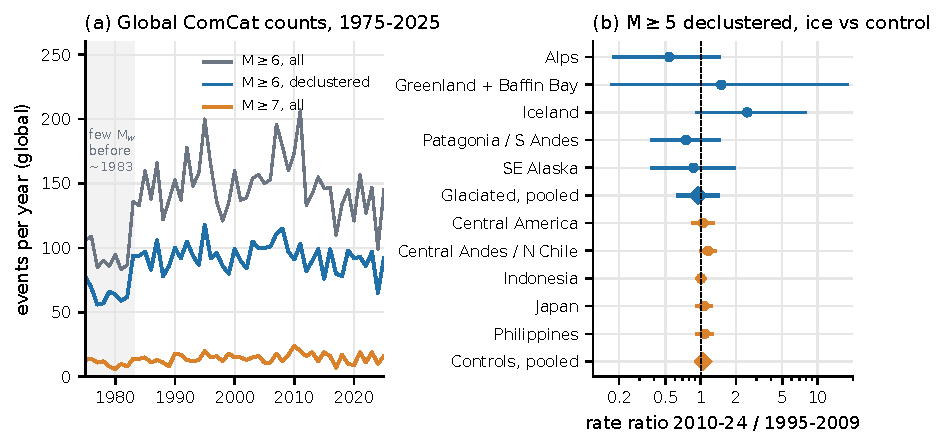
\includegraphics[width=\textwidth]{figures/fig01_global_baseline.pdf}
\caption{Exploratory global baseline. (a) ComCat global counts per year; shading marks the period with few moment magnitudes. (b) Declustered $M\geq5$ rate ratio 2010--2024 versus 1995--2009 with exact 95\,\% intervals; diamonds are pooled groups. West Antarctica (0 and 1 events) is omitted. Data: \texttt{results/global/}.}
\label{fig:global}
\end{figure}

\begin{table}[t]
\centering\small
\caption{Exploratory global and regional baseline. Data: \nolinkurl{results/global/global_trends.csv} and \nolinkurl{ice_vs_control_rate_ratios.csv}.}
\label{tab:global}
\begin{tabular}{lrll}
\toprule
Quantity & Estimate & 95\,\% interval & Note\\
\midrule
Trend $M\geq6$ all, 1990--2026 (\%/yr) & $-0.46$ & $-0.70$ to $-0.21$ & quasi: $-0.90$ to $-0.01$\\
Trend $M\geq6$ declustered (\%/yr) & $-0.31$ & $-0.62$ to $0.00$ & quasi: $-0.65$ to $+0.03$\\
Trend $M\geq7$ all (\%/yr) & $-0.21$ & $-0.99$ to $+0.57$ & \\
Glaciated pooled, $M\geq5$ decl.\ (60 $\to$ 57) & 0.95 & 0.65--1.39 & MDE 1.68\\
Control pooled, $M\geq5$ decl.\ (2679 $\to$ 2814) & 1.05 & 1.00--1.11 & MDE 1.08\\
Glaciated pooled, all events (83 $\to$ 151) & 1.82 & 1.38--2.41 & swarms, B\'ar{\dh}arbunga\\
GVP eruption starts, controls (223 $\to$ 235) & 1.05 & 0.87--1.27 & \\
\bottomrule
\end{tabular}
\end{table}

\subsection{Seasonal modulation in Southeast Alaska (F1, F2)}
SE Alaska has a strong and robust seasonal modulation: Schuster amplitude 0.112 ($p<10^{-6}$, $n=5164$), peak in mid-November, about one to two months after the maximum of GRACE unloading (load maximum in April) (Fig.~\ref{fig:seasonal}a). The load sensitivity is $\gamma_0=4.04\pm1.09$\,\%/kPa ($p=10^{-4}$), close to the 3.5\,\%/kPa reported by \textcite{johnson2020}. The in-network control Interior Alaska shows no seasonality (amplitude 0.023, $p=0.39$). Rain and load are correlated in SE Alaska ($r=0.68$) and cannot be separated (F3).

The amplitude is not growing significantly (Fig.~\ref{fig:seasonal}b, Fig.~\ref{fig:growth}): $\beta_1=+0.035\pm0.023$ per decade (95\,\% CI $-0.010$ to $+0.080$; one-sided Wald $p=0.064$, permutation $p=0.10$, BH $q=0.38$), and the load sensitivity declines insignificantly ($\gamma_1=-1.30\pm1.13$\,\%/kPa per decade, permutation $p=0.94$). Greenland has the largest growth estimate ($\beta_1=+0.146\pm0.088$, permutation $p=0.0055$, $q=0.083$) on a catalogue that densified strongly after 2008; Iceland is negative ($-0.096\pm0.063$). Among the controls, Japan's $\gamma_1$ is nominally significant ($p_\mathrm{perm}=0.021$, $q=0.29$). The inverse-variance mean of $\beta_1$ over the four national mountain regions is $0.033\pm0.015$ ($z=2.25$), but no glaciated-minus-control contrast in the criticality family is significant (Section~\ref{sec:crit}). With GK declustering the SE Alaska estimate is $+0.050\pm0.023$ (permutation $p=0.01$, uncorrected) \expl.

\begin{figure}[t]
\centering
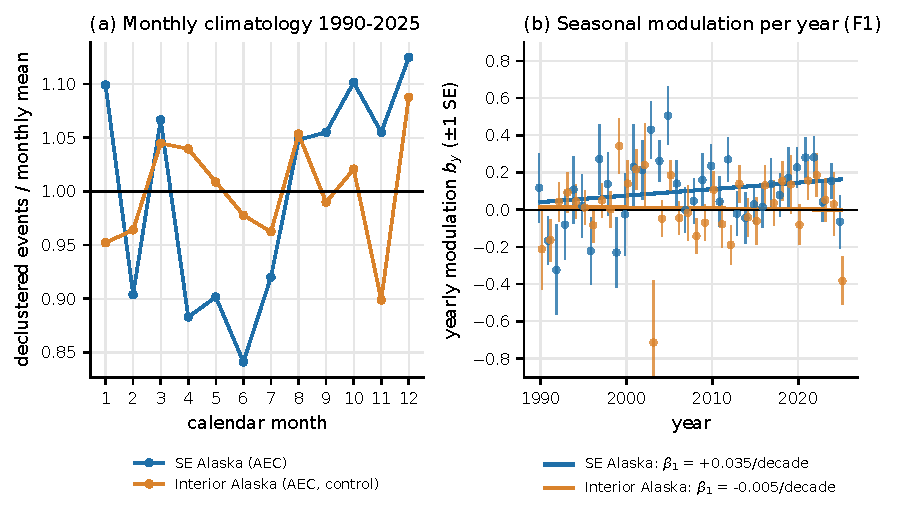
\includegraphics[width=\textwidth]{figures/fig02_seasonal_se_alaska.pdf}
\caption{Seasonality in SE Alaska. (a) Monthly climatology of declustered events, SE Alaska versus the Interior Alaska control. (b) Yearly modulation amplitude $b_y$ with the F1 fit. Data: \texttt{seasonal\_climatology.csv}, \texttt{F1\_per\_year\_modulation.csv}, \texttt{F1\_harmonic\_growth.csv}.}
\label{fig:seasonal}
\end{figure}

\begin{figure}[t]
\centering
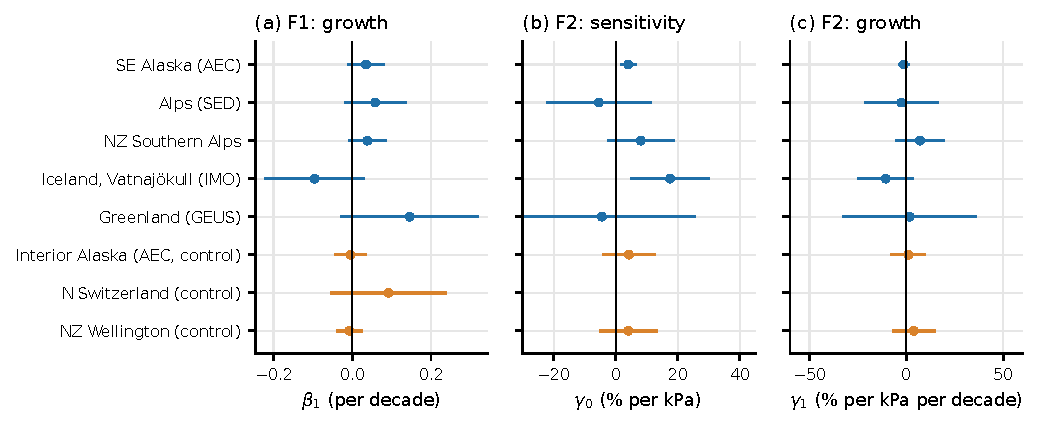
\includegraphics[width=\textwidth]{figures/fig03_growth_tests.pdf}
\caption{Pre-specified retrospective growth tests in the national-tier regions (95\,\% intervals; blue glaciated, orange controls). (a) F1 growth of seasonal amplitude; (b) F2 load sensitivity; (c) F2 growth of load sensitivity. N Switzerland has no GRACE signal and is omitted in (b, c). Data: \texttt{F1\_harmonic\_growth.csv}, \texttt{F2\_load\_sensitivity\_growth.csv}.}
\label{fig:growth}
\end{figure}

\begin{table}[t]
\centering\small
\caption{F1 and F2 for the national-tier regions (pre-specified, retrospective). $\beta_1$ per decade; $\gamma_0$ in \%/kPa; $\gamma_1$ in \%/kPa per decade; $p_\mathrm{perm}$ one-sided; $q$ BH over all regions.}
\label{tab:f1f2}
\begin{tabular}{lrrrrrr}
\toprule
Region & Schuster amp. & $\beta_1\pm$SE & $p_\mathrm{perm}$ & $q$ & $\gamma_0\pm$SE & $\gamma_1\pm$SE\\
\midrule
SE Alaska & 0.112 & $+0.035\pm0.023$ & 0.100 & 0.38 & $4.0\pm1.1$ & $-1.3\pm1.1$\\
Alps & 0.005 & $+0.058\pm0.039$ & 0.079 & 0.38 & $-5.5\pm8.5$ & $-2.5\pm9.5$\\
NZ Southern Alps & 0.035 & $+0.038\pm0.023$ & 0.058 & 0.38 & $8.1\pm5.3$ & $+7.1\pm6.2$\\
Iceland, Vatnaj\"okull & 0.299 & $-0.096\pm0.063$ & 0.861 & 0.86 & $17.6\pm6.3$ & $-10.6\pm7.1$\\
Greenland & 0.117 & $+0.146\pm0.088$ & 0.006 & 0.08 & $-4.5\pm15.2$ & $+1.7\pm17.3$\\
\midrule
Interior Alaska & 0.023 & $-0.005\pm0.020$ & 0.559 & 0.76 & $4.3\pm4.1$ & $+1.1\pm4.3$\\
N Switzerland & 0.071 & $+0.092\pm0.073$ & 0.132 & 0.40 & --- & ---\\
NZ Wellington & 0.001 & $-0.008\pm0.015$ & 0.709 & 0.82 & $4.0\pm4.6$ & $+3.9\pm5.3$\\
\bottomrule
\end{tabular}
\end{table}

\subsection{Criticality indicators}
\label{sec:crit}
Of 374 trend tests, 63 had $p<0.05$ and 10 survived BH; of 170 CSD tests 18 and 6; of 180 glaciated-versus-control group tests 2 and none (smallest $q=0.76$). The 16 BH hits are network and completeness effects (Mc trends, magnitude-type changes), $b$-value changes and variance increases that accompany rate increases or network densification (Greenland after about 2008); four of the ten trend hits are in control regions. Rising autocorrelation or falling recovery rate, the classical CSD signatures, are nowhere significant. Criticality is not excluded, but these indicators have little power with 18 two-year bins.

\subsection{ETAS background: H2.1 positive but not robust}
In stage 1 the Omori exponent ran to its lower bound ($p=1.0001$) in 7 of 8 regions, with branching ratios within the one-year kernel of 0.6--0.9. This is a serious diagnostic sign: model misfit (spatial heterogeneity, swarms, catalogue changes) is absorbed by a long tail, and long-range triggering beyond one year ends up in the background. Trend estimates are therefore model dependent.

The preregistered decision rule for H2.1 fired: SE Alaska's background trend ($+0.326\pm0.114$ per decade) exceeds Interior Alaska's ($-0.079\pm0.079$) by $+0.405\pm0.138$ ($z=2.93$, one-sided $p=0.0017$, BH 0.005; Table~\ref{tab:h2}). The effect, however, sits almost entirely in 1997--2002, when catalogue counts in both Alaska regions were very low and yearly $\Mc$ exceeded $\Mc^\mathrm{ref}$ (Fig.~\ref{fig:h21}a). Exploratory variants (Fig.~\ref{fig:h21}b): starting in 2003 the difference is $+0.11\pm0.16$; with a three-year triggering horizon $+0.23\pm0.21$; without 2025 $+0.41\pm0.15$; with a joint estimator $+0.43\pm0.13$ (from 2003 $+0.16$); with free Omori $p$ $+0.39\pm0.15$. Network covariates explain part of the trend: with FDSN station counts of all networks $+0.25\pm0.13$, permanent networks only $+0.38\pm0.10$, with $\Delta\Mc$ $+0.39\pm0.09$, complete years only $+0.37\pm0.10$ (OLS, no factor). Station metadata before 2000 are incomplete, so a network artefact is neither confirmed nor excluded. Together with the collapse from 2003 and the time-varying Mc, the result is better explained by a catalogue or model artefact than by a glacially driven background trend; H2.1 provides no evidence for a glacial contribution, though it does not exclude one. The secondary pairs are not significant (NZ $+0.095$, $p=0.19$; Alps $-0.350$).

\begin{figure}[t]
\centering
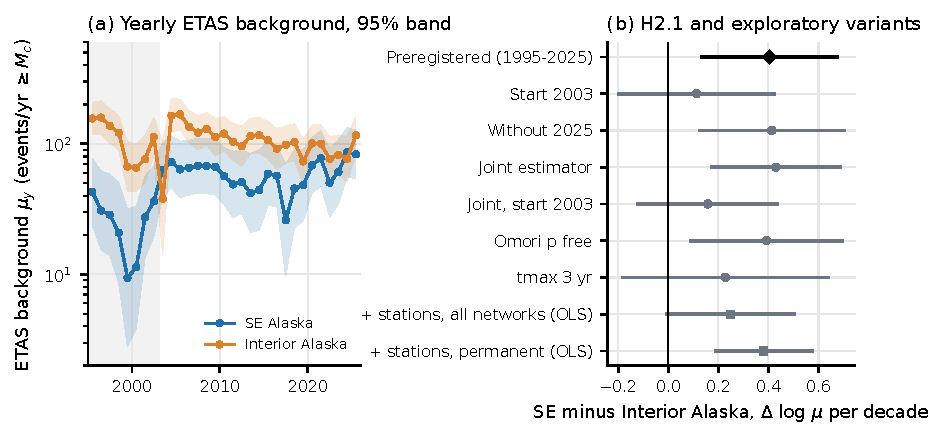
\includegraphics[width=\textwidth]{figures/fig04_h21_background.pdf}
\caption{H2.1. (a) Yearly ETAS residual background $\muy$ with 95\,\% band (SE inflated by the frozen factor 1.25); shading marks the low-count years before 2003. (b) Preregistered difference-in-differences of the background trend (black) and exploratory variants (grey; squares: OLS with station-count covariates). Data: \texttt{results/v02/m2\_*.csv}, \texttt{h21\_network\_models.csv}.}
\label{fig:h21}
\end{figure}

\begin{table}[t]
\centering\small
\caption{ETAS residual background (\texttt{m2\_etas\_background.csv}, \texttt{m2\_H21\_did.csv}). Trend of $\log\mu$ per decade (SE $\times$1.25); $\mu$ ratio 2020--2025 / 2008--2019 with 95\,\% interval; H2.2 class. Iceland and Greenland are descriptive.}
\label{tab:h2}
\begin{tabular}{lrrlr}
\toprule
Region & Trend / decade & $\mu$ ratio (95\,\%) & H2.2 class & Total ratio\\
\midrule
SE Alaska & $+0.326\pm0.114$ & 1.41 (1.07--1.85) & rise, not masked & 2.33\\
Interior Alaska & $-0.079\pm0.079$ & 0.87 (0.71--1.07) & no resolvable change & 0.91\\
NZ Southern Alps & $-0.326\pm0.059$ & 0.62 (0.45--0.86) & decrease (genuine quiet) & 0.32\\
NZ Wellington & $-0.421\pm0.091$ & 0.99 (0.67--1.47) & no resolvable change & 0.71\\
Alps & $-0.350\pm0.089$ & 1.22 (0.96--1.56) & no resolvable change & 1.30\\
N Switzerland & $+0.001\pm0.097$ & 1.94 (1.29--2.91) & rise, not masked & 2.04\\
Iceland, Vatnaj\"okull & $+0.194\pm0.144$ & 1.56 (0.85--2.86) & no resolvable change & 0.19\\
Greenland & $+1.047\pm0.207$ & 1.12 (0.75--1.67) & no resolvable change & 1.68\\
\midrule
\multicolumn{5}{l}{H2.1 primary: SE Alaska $-$ Interior: $+0.405\pm0.138$, $z=2.93$, $p_\text{one}=0.0017$, $p_\text{BH}=0.005$ \pre}\\
\bottomrule
\end{tabular}
\end{table}

\subsection{Masked background rise: H2.2}
No region meets the predefined ``masked background rise'' criterion (Table~\ref{tab:h2}). SE Alaska shows an unmasked rise (1.41) and N Switzerland a rise (1.94). The NZ Southern Alps quiet found in v0.1.0 is a genuine decrease of the residual background (0.62), but it disappears with EMR completeness ($\Mc=3.2$) and coincides with a joint step of both NZ regions in 2012, so a network effect is likely. Iceland comes closest to the pattern (total rate $-81$\,\%, $\mu$ $+56$\,\%), but the interval includes 1 and ETAS does not describe the swarms there. Rough 80\,\%-power thresholds are $\mu$ ratios of 1.3--2.4; the classification is descriptive and is mildly informative only against large masked rises in well-observed regions.

\subsection{Tides: H3}
Seismicity does not correlate significantly with the phase of the body-tide areal strain anywhere (Table~\ref{tab:tides}, Fig.~\ref{fig:tides}). In SE Alaska the amplitude is $a=0.042$ (Schuster $p=0.14$, BH 0.54); a modulation of $\geq6.8$\,\% relative to this phase would have been detected with 80\,\% power, and a $b$-value difference of $\geq0.07$. The smallest BH $q$ is 0.10 (Greenland, $\Delta b=-0.195$, one-sided $p=0.021$). Widening the extremum search to $\pm20$\,h changes no conclusion \expl.

\expl{} Ocean loading is comparable to or larger than the body tide in SE Alaska (RMS 19.9 versus 14.6\,nstrain) and Greenland (18.8 versus 11.9), and moves 20\,\% and 42\,\% of events into the other half-cycle. Tested against random times, the SE Alaska $p$ goes from 0.048 (body tide) to 0.081 (body plus ocean load); the Greenland $b$-value effect disappears ($p$ 0.023 $\to$ 0.58); the smallest BH $q$ with loading is 0.38. Fault-resolved Coulomb stress is not modelled, so the null applies to areal-strain phase only.

\begin{table}[t]
\centering\small
\caption{H3 body-tide tests \pre{} (\texttt{m3\_tides.csv}); last column exploratory ocean loading tested against random times \expl{} (\texttt{m3\_tides\_ocean\_load.csv}).}
\label{tab:tides}
\begin{tabular}{lrrrrrrr}
\toprule
Region & $N$ & $a$ & Schuster $p$ & $q$ & MDE $a$ & $\Delta b$ ($p_\text{one}$) & $p$ body+ocean\\
\midrule
SE Alaska & 4517 & 0.042 & 0.14 & 0.54 & 0.068 & $+0.023$ (0.79) & 0.081\\
NZ Southern Alps & 3665 & 0.006 & 0.97 & 0.99 & 0.072 & $+0.005$ (0.55) & 0.85\\
Alps & 1072 & 0.007 & 0.99 & 0.99 & 0.141 & $+0.097$ (0.86) & 0.87\\
Iceland, Vatnaj\"okull & 1227 & 0.071 & 0.22 & 0.54 & 0.126 & $-0.007$ (0.46) & 0.86\\
Greenland & 496 & 0.058 & 0.66 & 0.99 & 0.194 & $-0.195$ (0.021) & 0.81\\
\bottomrule
\end{tabular}
\end{table}

\begin{figure}[t]
\centering
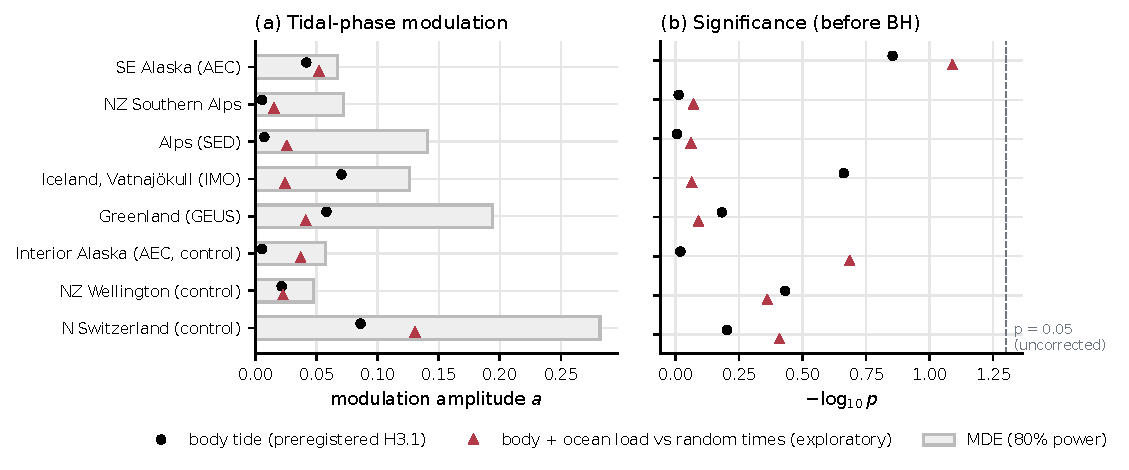
\includegraphics[width=\textwidth]{figures/fig05_tides.pdf}
\caption{Tidal-phase modulation. (a) Amplitude $a$ for the preregistered body-tide phase (dots) and the exploratory body-plus-ocean-load phase (triangles), with the 80\,\%-power MDE of the body-tide test (bars). (b) Uncorrected significance; the ocean-load test is against random times. Data: \texttt{results/v02/m3\_tides*.csv}.}
\label{fig:tides}
\end{figure}

\subsection{Lag model and tipping scenarios}
Relaxation times range from 23--117\,yr (Patagonia) and 64--170\,yr (SE Alaska) to 150--380\,yr (Iceland), 1000--2000\,yr (Alps) and about 4500\,yr (Fennoscandia reference). Narrow mountain loads are mostly answered elastically ($C=0.11$ in SE Alaska), broad ice-sheet loads mostly viscously ($C=0.94$ in SE Greenland). At constant present-day unloading, the viscously delayed rate increase is at most +19\,\% by 2036 and +27\,\% by 2100 even at $\kappa=1$ (+5\,\% or less with GRACE-box loads). A trend would be detectable in only 8 of 126 scenarios, the earliest around 2155.

Accelerating loss shortens this to decades (Table~\ref{tab:tipping}, Fig.~\ref{fig:tipping}). The earliest detectable increase is in SE Alaska under the SSP5-8.5 glacier path with glacier-surface loads (rate on promoted faults 1.21--2.35 by 2100, detection from 2045.8 in all four $\kappa$, $\dot S_0$ combinations). Amundsen paths become detectable around 2065--2079 only with a hypothetical dense network; SE Greenland stays within noise until about 2100. In the same framework the seasonal modulation \emph{falls} in all accelerating paths, to 0.43--0.97 of today by 2100, but this fall reaches at most $z=1.2$ with present catalogues. M4 \expl: viscosities and plate thicknesses informed by \textcite{sasgen2026} hardly move SE Alaska (earliest detection 2045.8 $\to$ 2047.3), because in this model the instantaneous share $1-C$ dominates; for Iceland $\tau$ shrinks from about 300 to 10\,yr and detection moves from 2070.3 to 2062.3.

\begin{table}[t]
\centering\small
\caption{Tipping scenarios (\texttt{tipping\_scenarios.csv}). Rate of promoted faults relative to 2025 (range over $\kappa\in\{0.3,1\}$, $\dot S_0\in\{10,30\}$\,kPa/yr) and earliest detection of an increase with present catalogue rates. Detection counts refer to the four promoted-fault runs ($f=0$). Model calculations, not forecasts.}
\label{tab:tipping}
\begin{tabular}{lccc}
\toprule
Region / path & 2050 & 2100 & Earliest detection (runs)\\
\midrule
SE Greenland, Edwards median & 1.00--1.03 & 1.01--1.10 & 2158 (1 of 4)\\
SE Greenland, Edwards 95th pct. & 1.00--1.04 & 1.02--1.24 & 2102 (3 of 4)\\
Amundsen, DeConto 3\,$^\circ$C (from 2060)$^\ast$ & 1.00--1.02 & 1.10--1.89 & 2079 (4 of 4)\\
Amundsen, DeConto early (from 2040)$^\ast$ & 1.01--1.06 & 1.11--1.96 & 2065 (4 of 4)\\
SE Alaska, glaciers SSP5-8.5 (surface) & 1.04--1.26 & 1.21--2.35 & 2046 (4 of 4)\\
SE Alaska, glaciers SSP5-8.5 (GRACE box) & 1.01--1.09 & 1.05--1.46 & 2061 (4 of 4)\\
Iceland, glaciers SSP5-8.5 (surface) & 1.03--1.19 & 1.13--1.99 & 2070 (4 of 4)\\
\bottomrule
\multicolumn{4}{l}{\footnotesize $^\ast$ hypothetical network with 100 events/yr; West Antarctica has no usable catalogue today.}
\end{tabular}
\end{table}

\begin{figure}[t]
\centering
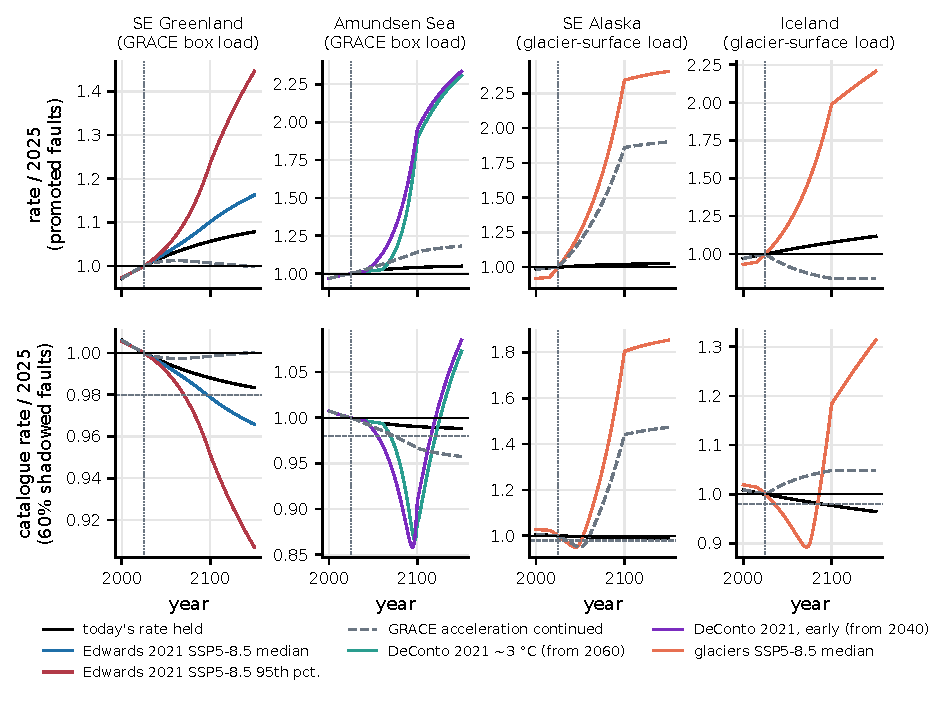
\includegraphics[width=\textwidth]{figures/fig06_tipping_quiet.pdf}
\caption{Tipping (top) and deceptive-quiet (bottom) scenarios for $\kappa=1$, $\dot S_0=10$\,kPa/yr. Top: rate of promoted faults relative to 2025. Bottom: catalogue rate with 60\,\% of faults in a stress shadow; the dashed line marks $-2$\,\%. Vertical dotted line: 2025. Data: \texttt{tipping\_curves.csv}.}
\label{fig:tipping}
\end{figure}

\subsection{Deceptive quiet before acceleration}
With 60\,\% of faults in a stress shadow, a quiet before the increase follows from the model (Fig.~\ref{fig:tipping}, bottom). It begins 7--59 years after the onset of acceleration in the Amundsen, SE Alaska and Iceland paths (45--93 years for the SE Greenland 95th-percentile path) but is shallow: the minimum catalogue rate is 0.84--0.96 of 2025 (4--16\,\%). With present catalogues it would become statistically detectable at the earliest around 2083; in the steepest paths (SE Alaska) it reverses (2053--2061) before it could be detected. Geodetic indicators respond directly to the load and would lead any seismic quiet.

Today, no region meets the frozen quiet rule except the NZ Southern Alps (Habermann $z=-2.5$, 109 $\to$ 89 events/yr), where the Wellington control in the same network also declines and the classification depends on $\Mc$. SE Alaska shows activation ($z=+3.1$, 161 $\to$ 194/yr). Iceland's ETAS-only signal coincides with a magnitude shift and the decay of the B\'ar{\dh}arbunga episode \parencite{habermann1991,sigmundsson2015}; on the load side Vatnaj\"okull loss is slowing, which corresponds to genuine relaxation rather than a deceptive quiet.

\subsection{Present-day precursors: GRACE and GNSS}
Only Patagonia exceeds the M1 threshold: $\xi=+0.039\pm0.007$/yr, loss rising from 19 to 34\,Gt/yr between 2002--2013 and 2014--2026 (Fig.~\ref{fig:precursors}a). Patagonia has no usable catalogue (ComCat is sparse and the relocated Chilean catalogue ends at 45.98$^\circ$S). Greenland ($\xi=-0.019\pm0.007$) and Vatnaj\"okull ($-0.022\pm0.007$) have been losing mass more slowly since about 2014 \parencite[cf.][]{bevis2019}; in the Amundsen Sea no significant acceleration is measurable \parencite[cf.][]{velicogna2020}. Four GNSS stations carry an M2 flag (Fig.~\ref{fig:precursors}b): TOMO (41.7\,mm/yr, acceleration $+2.31$\,mm/yr$^2$, $z=8.0$, consistent with \cite{barletta2018}), BACK ($z=4.9$), AB50 ($z=6.4$) and KELY ($z=8.3$). KELY is discordant with its slowing GRACE box and is reported, not interpreted, by rule.

\begin{figure}[t]
\centering
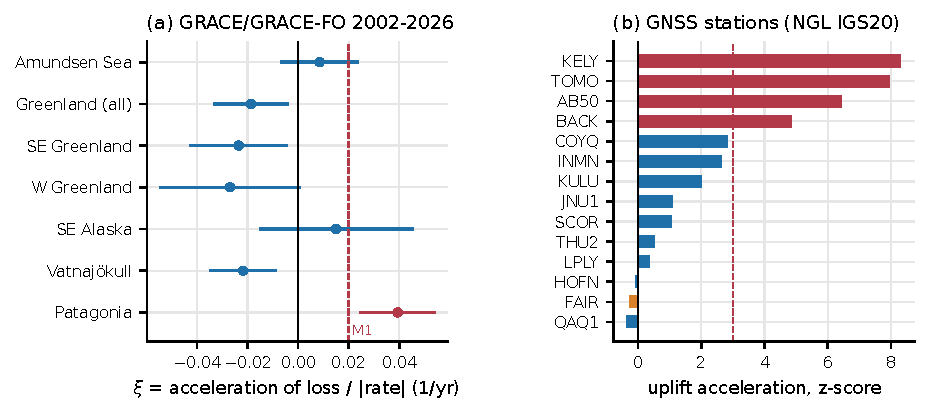
\includegraphics[width=\textwidth]{figures/fig07_precursors.pdf}
\caption{Monitoring precursors. (a) Normalised acceleration of GRACE mass loss $\xi$ with 95\,\% intervals and the frozen M1 threshold. (b) GNSS uplift acceleration $z$ (red: M2 flag; orange: control station FAIR). Data: \texttt{precursors\_grace\_acceleration.csv}, \texttt{precursors\_gnss\_uplift.csv}.}
\label{fig:precursors}
\end{figure}

%==========================================================================================
\section{Review process and errata}
\label{sec:review}
Version 0.2 was reviewed in one round by several AI systems, each with a written brief (\nolinkurl{docs/REVIEW_PROMPTS.md}): a ``Deep Research'' scientific review (DR), a preregistration audit by Grok (GR), a full code review with independent scripts and simulations by Claude Code (CC), a pull-request comment by Codex (CX), a narrow literature check by Gemini (GE; used as an idea source only) and the ETAS likelihood and simulator checks by Grok Bot (GB). Raw reviews are archived in \texttt{docs/reviews/raw/} (except GE), and all 41 points with verdicts and actions are listed in \texttt{docs/reviews/REVIEW\_RESPONSE\_v0.2.md}. New literature claims from reviews were checked against primary sources before adoption; one GE objection (Sasgen values ``not found'') was rejected after checking the paper.

\paragraph{Erratum E1.} CX and CC independently found that the null calibration of the H2 standard-error factor 1.25 used a half-open window function with the wrong windows (2008--2018 versus 2020--2024) and a geometry without the five-year lead-in. Re-run in production geometry (CC and GB), the factor is sufficient for the trend test; for the window ratio a factor of about 1.2--1.4 would be needed. In the repository's calibration runs (\texttt{calibration\_summary.csv}) the trend $\mathrm{sd}(z)$ is 0.96--1.07 (90\,\% upper bounds 1.07--1.22) and the window-ratio $\mathrm{sd}(z)$ 1.18--1.24 (upper bounds 1.27--1.35); the addendum quotes up to 1.30 and 1.42 including the reviewers' own runs, which are not archived. No published decision changes below a factor of 1.56. The frozen value stays (A5); the H2.2 intervals should be read as somewhat too narrow.

\paragraph{Other corrections.} Simulator fixes (division by zero at $p=1$; magnitude discretisation that gave $b\approx0.90$ instead of 1, now 0.997) affected only simulations; the recovery study was re-run with qualitatively unchanged results. The C2 SE factor ambiguity was clarified (A1), look dates were made robust (A3), and the origin of the frozen Love numbers was traced to SPOTL's body-tide values. Wording was sharpened where DR showed that interpretations went beyond the estimand: $\muy$ is a residual background; H3 tests the body-tide areal-strain phase only; the lag model is a thin-plate/half-space sensitivity, not a reproduction of the \textcite{sasgen2026} rheology. After v0.2.0 the global baseline script was made deterministic for magnitude ties, which moved the declustered $M\geq6$ trend from $-0.29$ to $-0.31$\,\%/yr and the pooled glaciated ratio from 0.93 to 0.95 \expl.

%==========================================================================================
\section{Discussion}
\label{sec:discussion}

\paragraph{What the data exclude.}
At the global scale, a rise of the declustered $M\geq6$ rate faster than about 0.03\,\%/yr since 1990 is incompatible with ComCat. Pooled over glaciated boxes, a rise of the declustered $M\geq5$ rate by more than about 40\,\% between 1995--2009 and 2010--2024 is unlikely (upper bound 1.39). In SE Alaska a growth of the seasonal amplitude faster than about 0.08 per decade (upper 95\,\% bound; today's amplitude is about 0.10) and a body-tide modulation larger than about 7\,\% would probably have been seen. No region shows a large masked background rise.

\paragraph{What remains open.}
Moderate changes are not excluded anywhere. Single glaciated regions can only resolve rate ratios of 2.4--3.5, Iceland and Greenland catalogues are too heterogeneous for background trends, Patagonia (the one region with accelerating loss) and West Antarctica lack usable catalogues, and ocean-load and fault-resolved stresses are only partly modelled. The positive but non-robust H2.1 result shows how a preregistered test without a start-year check can hinge on a network phase; C2 starts in a homogeneous network period and carries explicit homogeneity rules.

\paragraph{An early-stage hypothesis.}
Taken together, the evidence is compatible with a hypothesis in an early stage: present-day ice loss may change the seismic response of glaciated regions, but if it does, the change is currently below what the catalogues can resolve, and the scenario calculations suggest it will remain so for decades unless loss accelerates strongly. We do not claim a glacially driven change, and we do not claim its absence.

\paragraph{Rate-and-state implication.}
A growing seasonal modulation would not be the generic expectation of accelerated unloading. In Dieterich's model, for loading periods much longer than the aftershock duration the relative modulation scales as $\Delta S/(T\dot S)$, so additional GIA stressing \emph{lowers} it (our scenarios: to 0.43--0.97 of today by 2100). If the modulation grew, more likely explanations would be a falling effective normal stress (pore pressure, as suggested for Mont Blanc by \cite{simon2025}) or faults approaching failure, as discussed for Parkfield by \textcite{sirorattanakul2026}. This is why F1 alone could never show causality, and why C1 tests modulation growth as a sign of changing fault conditions rather than of unloading per se.

%==========================================================================================
\section{Limitations}
\label{sec:limitations}
\begin{itemize}
  \item Retrospective tests use data examined before the rules were fixed; only C1 and C2 are independent.
  \item Catalogues change networks, magnitude types and completeness; in-network controls do not protect against differential network changes. Station metadata before about 2000 are incomplete.
  \item The temporal ETAS model has no spatial kernel; $p$ at its lower bound in 7 of 8 regions makes levels and trends model dependent; H2 SEs are conditional on stage-1 parameters (propagation adds about 1--2\,\%).
  \item GRACE resolution (about 300\,km) smears narrow mountain loads; rain and load are not separable in SE Alaska.
  \item Tidal tests use areal-strain phase at cell centroids; TPXO\,7.2 resolves fjords poorly; no fault-resolved stress.
  \item The lag and tipping models are reduced (half-space plus plate, unconstrained coupling $\kappa$, assumed shadow fraction); their numbers are scenario properties, not forecasts.
  \item The global baseline is exploratory, uses rectangular boxes and coarse declustering; declustered counts carry method uncertainty beyond Poisson intervals.
  \item The analysis was carried out by one person with AI assistance; reviews were by AI systems, not by independent human experts.
\end{itemize}

%==========================================================================================
\section{Conclusions}
\label{sec:conclusions}
\begin{enumerate}
  \item There is no sign of a global or pooled glaciated increase of declustered seismicity, with upper bounds of about 0.03\,\%/yr (global $M\geq6$) and a rate ratio of 1.39 (pooled glaciated $M\geq5$).
  \item SE Alaska is seasonally modulated (4\,\%/kPa), but the modulation is not demonstrably growing.
  \item The one formally positive preregistered test (H2.1) is not robust and is most plausibly a catalogue artefact.
  \item Tidal, quiescence and criticality tests are null, with stated MDEs.
  \item Physical scenarios place detectable effects decades ahead and predict a shallow quiet before acceleration; geodetic indicators would lead.
  \item Two prospective tests are frozen and will be evaluated in 2029 and 2036; their power is limited, and this was stated in advance.
\end{enumerate}

%==========================================================================================
\section*{Author contributions and use of AI}
J.\,B.\,R. (independent researcher; certified IT specialist for application development with a background in web design) conceived the project, set the research questions and decision rules, approved every preregistration and addendum, and is responsible for all scientific claims. The work was developed using AI-assisted research methods as collaborative tools under direct human oversight: data retrieval, analysis code, figures, documentation and drafts of this manuscript were produced with an AI agent (Grok Bot) on the author's instructions; the review round used further AI systems (Deep Research, Grok, Claude Code, Codex; Gemini as an idea source only), whose raw reports are archived and whose points were checked against code, data and primary literature before adoption. The collaboration between the author and these AI systems runs under the informal working name ``MOR collective'', which is not a legal entity or institution. No AI system is an author. All scientific claims and methodological decisions are the responsibility of the human author.

\section*{Data and code availability}
Code, frozen files, result tables and documentation: GitHub \url{https://github.com/GenesisAeon/glacial-seismic-sensitivity-utac}; archived releases v0.1.0 (\href{https://doi.org/10.5281/zenodo.23281091}{10.5281/zenodo.23281091}) and v0.2.0 (\href{https://doi.org/10.5281/zenodo.23286492}{10.5281/zenodo.23286492}); concept DOI \href{https://doi.org/10.5281/zenodo.23281090}{10.5281/zenodo.23281090}; Python package \url{https://pypi.org/project/glacial-seismic-sensitivity-utac/}. Figures in this paper are re-rendered from the CSV files in \texttt{results/} by \texttt{paper/figures/make\_paper\_figures.py}. All input data are public (Section~\ref{sec:data}); global snapshots are archived in \texttt{results/global/snapshots/}. The project is registered as P133 (KLIMA-KRYO-13) in the GenesisAeon research programme.

\section*{Funding}
This work received no external funding; the author is independent and self-funded.

\section*{Competing interests}
The author declares no competing interests.

\printbibliography[heading=bibintoc]

\end{document}
